
%% bare_conf.tex
%% V1.3
%% 2007/01/11
%% by Michael Shell
%% See:
%% http://www.michaelshell.org/
%% for current contact information.
%%
%% This is a skeleton file demonstrating the use of IEEEtran.cls
%% (requires IEEEtran.cls version 1.7 or later) with an IEEE conference paper.
%%
%% Support sites:
%% http://www.michaelshell.org/tex/ieeetran/
%% http://www.ctan.org/tex-archive/macros/latex/contrib/IEEEtran/
%% and
%% http://www.ieee.org/

%%*************************************************************************
%% Legal Notice:
%% This code is offered as-is without any warranty either expressed or
%% implied; without even the implied warranty of MERCHANTABILITY or
%% FITNESS FOR A PARTICULAR PURPOSE! 
%% User assumes all risk.
%% In no event shall IEEE or any contributor to this code be liable for
%% any damages or losses, including, but not limited to, incidental,
%% consequential, or any other damages, resulting from the use or misuse
%% of any information contained here.
%%
%% All comments are the opinions of their respective authors and are not
%% necessarily endorsed by the IEEE.
%%
%% This work is distributed under the LaTeX Project Public License (LPPL)
%% ( http://www.latex-project.org/ ) version 1.3, and may be freely used,
%% distributed and modified. A copy of the LPPL, version 1.3, is included
%% in the base LaTeX documentation of all distributions of LaTeX released
%% 2003/12/01 or later.
%% Retain all contribution notices and credits.
%% ** Modified files should be clearly indicated as such, including  **
%% ** renaming them and changing author support contact information. **
%%
%% File list of work: IEEEtran.cls, IEEEtran_HOWTO.pdf, bare_adv.tex,
%%                    bare_conf.tex, bare_jrnl.tex, bare_jrnl_compsoc.tex
%%*************************************************************************

% *** Authors should verify (and, if needed, correct) their LaTeX system  ***
% *** with the testflow diagnostic prior to trusting their LaTeX platform ***
% *** with production work. IEEE's font choices can trigger bugs that do  ***
% *** not appear when using other class files.                            ***
% The testflow support page is at:
% http://www.michaelshell.org/tex/testflow/



% Note that the a4paper option is mainly intended so that authors in
% countries using A4 can easily print to A4 and see how their papers will
% look in print - the typesetting of the document will not typically be
% affected with changes in paper size (but the bottom and side margins will).
% Use the testflow package mentioned above to verify correct handling of
% both paper sizes by the user's LaTeX system.
%
% Also note that the "draftcls" or "draftclsnofoot", not "draft", option
% should be used if it is desired that the figures are to be displayed in
% draft mode.
%
\documentclass[conference, cmex10]{IEEEtran}
\usepackage{amsmath, graphicx, blindtext, tikz, csvsimple}
\usepackage{amsfonts}
\usepackage{amssymb}
\interdisplaylinepenalty=2500
\usepackage{tikzscale, adjustbox}
\usepackage[school]{pgf-umlcd}
\usepackage{algorithm2e}
\usepackage{verbatim} 
\usepackage{booktabs} % For \toprule, \midrule and \bottomrule
\usepackage{siunitx} % Formats the units and values
\usepackage{pgfplotstable} % Generates table from .csv

% Setup siunitx:
\sisetup{
  round-mode          = places, % Rounds numbers
  round-precision     = 2, % to 2 places
}

%\usepackage[a4paper,margin=1cm,landscape]{geometry}
\usetikzlibrary{mindmap, positioning,shapes,shadows,arrows}

% Add the compsoc option for Computer Society conferences.
%
% If IEEEtran.cls has not been installed into the LaTeX system files,
% manually specify the path to it like:
% \documentclass[conference]{../sty/IEEEtran}





% Some very useful LaTeX packages include:
% (uncomment the ones you want to load)


% *** MISC UTILITY PACKAGES ***
%
%\usepackage{ifpdf}
% Heiko Oberdiek's ifpdf.sty is very useful if you need conditional
% compilation based on whether the output is pdf or dvi.
% usage:
% \ifpdf
%   % pdf code
% \else
%   % dvi code
% \fi
% The latest version of ifpdf.sty can be obtained from:
% http://www.ctan.org/tex-archive/macros/latex/contrib/oberdiek/
% Also, note that IEEEtran.cls V1.7 and later provides a builtin
% \ifCLASSINFOpdf conditional that works the same way.
% When switching from latex to pdflatex and vice-versa, the compiler may
% have to be run twice to clear warning/error messages.






% *** CITATION PACKAGES ***
%
%\usepackage{cite}
% cite.sty was written by Donald Arseneau
% V1.6 and later of IEEEtran pre-defines the format of the cite.sty package
% \cite{} output to follow that of IEEE. Loading the cite package will
% result in citation numbers being automatically sorted and properly
% "compressed/ranged". e.g., [1], [9], [2], [7], [5], [6] without using
% cite.sty will become [1], [2], [5]--[7], [9] using cite.sty. cite.sty's
% \cite will automatically add leading space, if needed. Use cite.sty's
% noadjust option (cite.sty V3.8 and later) if you want to turn this off.
% cite.sty is already installed on most LaTeX systems. Be sure and use
% version 4.0 (2003-05-27) and later if using hyperref.sty. cite.sty does
% not currently provide for hyperlinked citations.
% The latest version can be obtained at:
% http://www.ctan.org/tex-archive/macros/latex/contrib/cite/
% The documentation is contained in the cite.sty file itself.






% *** GRAPHICS RELATED PACKAGES ***
%
\ifCLASSINFOpdf
  % \usepackage[pdftex]{graphicx}
  % declare the path(s) where your graphic files are
  % \graphicspath{{../pdf/}{../jpeg/}}
  % and their extensions so you won't have to specify these with
  % every instance of \includegraphics
  % \DeclareGraphicsExtensions{.pdf,.jpeg,.png}
\else
  % or other class option (dvipsone, dvipdf, if not using dvips). graphicx
  % will default to the driver specified in the system graphics.cfg if no
  % driver is specified.
  % \usepackage[dvips]{graphicx}
  % declare the path(s) where your graphic files are
  % \graphicspath{{../eps/}}
  % and their extensions so you won't have to specify these with
  % every instance of \includegraphics
  % \DeclareGraphicsExtensions{.eps}
\fi
% graphicx was written by David Carlisle and Sebastian Rahtz. It is
% required if you want graphics, photos, etc. graphicx.sty is already
% installed on most LaTeX systems. The latest version and documentation can
% be obtained at: 
% http://www.ctan.org/tex-archive/macros/latex/required/graphics/
% Another good source of documentation is "Using Imported Graphics in
% LaTeX2e" by Keith Reckdahl which can be found as epslatex.ps or
% epslatex.pdf at: http://www.ctan.org/tex-archive/info/
%
% latex, and pdflatex in dvi mode, support graphics in encapsulated
% postscript (.eps) format. pdflatex in pdf mode supports graphics
% in .pdf, .jpeg, .png and .mps (metapost) formats. Users should ensure
% that all non-photo figures use a vector format (.eps, .pdf, .mps) and
% not a bitmapped formats (.jpeg, .png). IEEE frowns on bitmapped formats
% which can result in "jaggedy"/blurry rendering of lines and letters as
% well as large increases in file sizes.
%
% You can find documentation about the pdfTeX application at:
% http://www.tug.org/applications/pdftex





% *** MATH PACKAGES ***
%
\usepackage{amsmath}
% A popular package from the American Mathematical Society that provides
% many useful and powerful commands for dealing with mathematics. If using
% it, be sure to load this package with the cmex10 option to ensure that
% only type 1 fonts will utilized at all point sizes. Without this option,
% it is possible that some math symbols, particularly those within
% footnotes, will be rendered in bitmap form which will result in a
% document that can not be IEEE Xplore compliant!
%
% Also, note that the amsmath package sets \interdisplaylinepenalty to 10000
% thus preventing page breaks from occurring within multiline equations. Use:
%\interdisplaylinepenalty=2500
% after loading amsmath to restore such page breaks as IEEEtran.cls normally
% does. amsmath.sty is already installed on most LaTeX systems. The latest
% version and documentation can be obtained at:
% http://www.ctan.org/tex-archive/macros/latex/required/amslatex/math/





% *** SPECIALIZED LIST PACKAGES ***
%
%\usepackage{algorithmic}
% algorithmic.sty was written by Peter Williams and Rogerio Brito.
% This package provides an algorithmic environment fo describing algorithms.
% You can use the algorithmic environment in-text or within a figure
% environment to provide for a floating algorithm. Do NOT use the algorithm
% floating environment provided by algorithm.sty (by the same authors) or
% algorithm2e.sty (by Christophe Fiorio) as IEEE does not use dedicated
% algorithm float types and packages that provide these will not provide
% correct IEEE style captions. The latest version and documentation of
% algorithmic.sty can be obtained at:
% http://www.ctan.org/tex-archive/macros/latex/contrib/algorithms/
% There is also a support site at:
% http://algorithms.berlios.de/index.html
% Also of interest may be the (relatively newer and more customizable)
% algorithmicx.sty package by Szasz Janos:
% http://www.ctan.org/tex-archive/macros/latex/contrib/algorithmicx/




% *** ALIGNMENT PACKAGES ***
%
%\usepackage{array}
% Frank Mittelbach's and David Carlisle's array.sty patches and improves
% the standard LaTeX2e array and tabular environments to provide better
% appearance and additional user controls. As the default LaTeX2e table
% generation code is lacking to the point of almost being broken with
% respect to the quality of the end results, all users are strongly
% advised to use an enhanced (at the very least that provided by array.sty)
% set of table tools. array.sty is already installed on most systems. The
% latest version and documentation can be obtained at:
% http://www.ctan.org/tex-archive/macros/latex/required/tools/


%\usepackage{mdwmath}
%\usepackage{mdwtab}
% Also highly recommended is Mark Wooding's extremely powerful MDW tools,
% especially mdwmath.sty and mdwtab.sty which are used to format equations
% and tables, respectively. The MDWtools set is already installed on most
% LaTeX systems. The lastest version and documentation is available at:
% http://www.ctan.org/tex-archive/macros/latex/contrib/mdwtools/


% IEEEtran contains the IEEEeqnarray family of commands that can be used to
% generate multiline equations as well as matrices, tables, etc., of high
% quality.


%\usepackage{eqparbox}
% Also of notable interest is Scott Pakin's eqparbox package for creating
% (automatically sized) equal width boxes - aka "natural width parboxes".
% Available at:
% http://www.ctan.org/tex-archive/macros/latex/contrib/eqparbox/





% *** SUBFIGURE PACKAGES ***
%\usepackage[tight,footnotesize]{subfigure}
% subfigure.sty was written by Steven Douglas Cochran. This package makes it
% easy to put subfigures in your figures. e.g., "Figure 1a and 1b". For IEEE
% work, it is a good idea to load it with the tight package option to reduce
% the amount of white space around the subfigures. subfigure.sty is already
% installed on most LaTeX systems. The latest version and documentation can
% be obtained at:
% http://www.ctan.org/tex-archive/obsolete/macros/latex/contrib/subfigure/
% subfigure.sty has been superceeded by subfig.sty.



%\usepackage[caption=false]{caption}
%\usepackage[font=footnotesize]{subfig}
% subfig.sty, also written by Steven Douglas Cochran, is the modern
% replacement for subfigure.sty. However, subfig.sty requires and
% automatically loads Axel Sommerfeldt's caption.sty which will override
% IEEEtran.cls handling of captions and this will result in nonIEEE style
% figure/table captions. To prevent this problem, be sure and preload
% caption.sty with its "caption=false" package option. This is will preserve
% IEEEtran.cls handing of captions. Version 1.3 (2005/06/28) and later 
% (recommended due to many improvements over 1.2) of subfig.sty supports
% the caption=false option directly:
%\usepackage[caption=false,font=footnotesize]{subfig}
%
% The latest version and documentation can be obtained at:
% http://www.ctan.org/tex-archive/macros/latex/contrib/subfig/
% The latest version and documentation of caption.sty can be obtained at:
% http://www.ctan.org/tex-archive/macros/latex/contrib/caption/




% *** FLOAT PACKAGES ***
%
%\usepackage{fixltx2e}
% fixltx2e, the successor to the earlier fix2col.sty, was written by
% Frank Mittelbach and David Carlisle. This package corrects a few problems
% in the LaTeX2e kernel, the most notable of which is that in current
% LaTeX2e releases, the ordering of single and double column floats is not
% guaranteed to be preserved. Thus, an unpatched LaTeX2e can allow a
% single column figure to be placed prior to an earlier double column
% figure. The latest version and documentation can be found at:
% http://www.ctan.org/tex-archive/macros/latex/base/



%\usepackage{stfloats}
% stfloats.sty was written by Sigitas Tolusis. This package gives LaTeX2e
% the ability to do double column floats at the bottom of the page as well
% as the top. (e.g., "\begin{figure*}[!b]" is not normally possible in
% LaTeX2e). It also provides a command:
%\fnbelowfloat
% to enable the placement of footnotes below bottom floats (the standard
% LaTeX2e kernel puts them above bottom floats). This is an invasive package
% which rewrites many portions of the LaTeX2e float routines. It may not work
% with other packages that modify the LaTeX2e float routines. The latest
% version and documentation can be obtained at:
% http://www.ctan.org/tex-archive/macros/latex/contrib/sttools/
% Documentation is contained in the stfloats.sty comments as well as in the
% presfull.pdf file. Do not use the stfloats baselinefloat ability as IEEE
% does not allow \baselineskip to stretch. Authors submitting work to the
% IEEE should note that IEEE rarely uses double column equations and
% that authors should try to avoid such use. Do not be tempted to use the
% cuted.sty or midfloat.sty packages (also by Sigitas Tolusis) as IEEE does
% not format its papers in such ways.





% *** PDF, URL AND HYPERLINK PACKAGES ***
%
%\usepackage{url}
% url.sty was written by Donald Arseneau. It provides better support for
% handling and breaking URLs. url.sty is already installed on most LaTeX
% systems. The latest version can be obtained at:
% http://www.ctan.org/tex-archive/macros/latex/contrib/misc/
% Read the url.sty source comments for usage information. Basically,
% \url{my_url_here}.





% *** Do not adjust lengths that control margins, column widths, etc. ***
% *** Do not use packages that alter fonts (such as pslatex).         ***
% There should be no need to do such things with IEEEtran.cls V1.6 and later.
% (Unless specifically asked to do so by the journal or conference you plan
% to submit to, of course. )


% correct bad hyphenation here
%\hyphenation{op-tical net-works semi-conduc-tor}




\begin{document}
%
% paper title
% can use linebreaks \\ within to get better formatting as desired
\title{Fixed-Size Least Squares Support Vector Machines: Scalable Implementation for Large Scale Predictive Models}


% author names and affiliations
% use a multiple column layout for up to three different
% affiliations
\author{\IEEEauthorblockN{Mandar Chandorkar\IEEEauthorrefmark{1}, Oliver Lauwers, Raghvendra Mall, Johan A.K Suykens, Bart De Moor}

\IEEEauthorblockA{\IEEEauthorrefmark{1} ESAT-STADIUS KU Leuven \\ Kasteelpark Arenberg 10, \\ 
B-3001 Leuven, Belgium}}
% conference papers do not typically use \thanks and this command
% is locked out in conference mode. If really needed, such as for
% the acknowledgment of grants, issue a \IEEEoverridecommandlockouts
% after \documentclass

% for over three affiliations, or if they all won't fit within the width
% of the page, use this alternative format:
% 
%\author{\IEEEauthorblockN{Michael Shell\IEEEauthorrefmark{1},
%Homer Simpson\IEEEauthorrefmark{2},
%James Kirk\IEEEauthorrefmark{3}, 
%Montgomery Scott\IEEEauthorrefmark{3} and
%Eldon Tyrell\IEEEauthorrefmark{4}}
%\IEEEauthorblockA{\IEEEauthorrefmark{1}School of Electrical and Computer Engineering\\
%Georgia Institute of Technology,
%Atlanta, Georgia 30332--0250\\ Email: see http://www.michaelshell.org/contact.html}
%\IEEEauthorblockA{\IEEEauthorrefmark{2}Twentieth Century Fox, Springfield, USA\\
%Email: homer@thesimpsons.com}
%\IEEEauthorblockA{\IEEEauthorrefmark{3}Starfleet Academy, San Francisco, California 96678-2391\\
%Telephone: (800) 555--1212, Fax: (888) 555--1212}
%\IEEEauthorblockA{\IEEEauthorrefmark{4}Tyrell Inc., 123 Replicant Street, Los Angeles, California 90210--4321}}




% use for special paper notices
%\IEEEspecialpapernotice{(Invited Paper)}




% make the title area
\maketitle


\begin{abstract}
%\boldmath
 We propose \textit{DynaML}, a flexible and modular \textit{Scala} based library for the implementing and tuning large scale supervised kernel based models. The framework consists of a set of modules for (gradient and gradient free) optimization, model representation, kernel functions, evaluation and probabilistic graphical models.
 
 A kernel based \emph{Fixed-Size Least Squares Support Vector Machine} (FS-LSSVM) model is implemented using the proposed framework, while heavily leveraging the parallel computing capabilities of \textit{Apache Spark}. Global optimization routines like \emph{Coupled Simulated Annealing} (CSA) and \emph{Grid Search} are implemented in the optimization module and are used to tune the hyper-parameters of the FS-LSSVM model. Finally, we carry out experiments on standard data sets like \emph{Magic Gamma}, \emph{Ripley}, \emph{Forest Cover}, \emph{Susy} etc. and evaluate the performance of various kernel in combination with LSSVMs.     

\end{abstract}
% IEEEtran.cls defaults to using nonbold math in the Abstract.
% This preserves the distinction between vectors and scalars. However,
% if the journal you are submitting to favors bold math in the abstract,
% then you can use LaTeX's standard command \boldmath at the very start
% of the abstract to achieve this. Many IEEE journals frown on math
% in the abstract anyway.

% Note that keywords are not normally used for peerreview papers.
\begin{IEEEkeywords}
FS-LSSVM, Big Data, Large Scale Models, Non-linear SVMs
\end{IEEEkeywords}






% For peer review papers, you can put extra information on the cover
% page as needed:
% \ifCLASSOPTIONpeerreview
% \begin{center} \bfseries EDICS Category: 3-BBND \end{center}
% \fi
%
% For peerreview papers, this IEEEtran command inserts a page break and
% creates the second title. It will be ignored for other modes.
\IEEEpeerreviewmaketitle



\section{Introduction} \label{introduction}
The $21^{st}$ century stands out in how mankind learned the value of storing and making predictions/decisions from large volumes of data. A significant aspect of large scale data analysis is distributed computation frameworks like \textit{High Performance Computing}, \textit{Message Passing Interface} etc. Recently large scale commodity hardware clusters have replaced the two former frameworks as the most popular model for parallel data analysis. With this crucial change in hardware came a change in computational models as well. It is at this juncture that distributed \textit{Map Reduce} became the de-facto computational philosophy for large scale data analysis and  words such as \textit{Hadoop} \cite{Hadoop:2005}, \cite{chang2008bigtable}, \cite{Borthakur2011} and \textit{Apache Spark} \cite{Zaharia2010}, \cite{Spark:2010} have become synonymous with large scale data analysis and machine learning.

Along with innovation in hardware design and distributed computing models, there came a need for good programming libraries and frameworks to work with various Machine Learning models on large data sets. It was demonstrated in \cite{10.1109/MIS.2009.36} that a gigantic language corpus encapsulates almost all aspects of human language and speech. So far the prevalent `motto' in the Internet industry has been ``large data, simple models", which is a mis-understood phrase as it can be confused as a statement of \textit{Occam's Razor}. The decomposition of the generalization error in Machine Learning is the well known ``bias-variance" trade-off \cite{Valentini2004}, from that it can be observed that there is an optimal point between the bias and variance of a model such that the generalization error is minimum.

Therefore, in order to extract maximum value from large scale data, it is imperative to have the flexibility to train and compare different model families before arriving at the one that fits the requirement of the user. This is not possible in a rigid, monolithic programming framework. Modularity, extensibility and ease of usage are of paramount importance while designing Machine Learning software for large scale data applications. In the sections that follow, we review the \textit{Fixed-Size Least Squares Support Vector Machine} (FS-LSSVM) algorithm as outlined by the authors in \cite{DeBrabanter2010} and give an introduction to \textit{DynaML} and its component modules.

\section*{DynaML}
Our library tackles three major issues w.r.t. the design of a Machine Learning research toolkit.

\begin{itemize}
\item \textbf{Modularity}:
It is imperative in data science to tweak models by changing the various components which they employ to learn, for example a model may be linear or kernel based, it can be optimized by various methods like \textit{Stochastic Gradient Descent}, \textit{Conjugate Gradient}, etc, there may be a mechanism of model selection or hyper-parameter optimization. Keeping the source code modular enables quick development and tuning of advanced models which build on a set of common building blocks.
\item \textbf{Flexibility of Abstraction}:
Learning models employ various mathematical structures; graphs, vectors, matrices etc. They also have a hierarchy which defines their parameters, objective functions and by extension their behavior. By representing learning models based on a abstract class hierarchy, our library leverages \textit{Object Oriented Programming} to create a powerful and reusable code base.
\item \textbf{Distributed Computing/Database Support}:
The big data landscape has many tools which enable the storage and analysis of large streams of data, they consist of technologies such as, but not limited to \textit{Apache Spark}, \textit{Hadoop}, Graph Databases like \textit{Titan} \cite{Titan:2014}, \textit{OrientDB} \cite{OrientDB:2010}, \textit{Neo4j} \cite{Neo4j:2010}. Creating a powerful framework for model training and evaluation requires the decoupling of storage and processing infrastructure from the actual logic that implements the architecture of learning models.
\end{itemize}

In the following section we introduce the FS-LSSVM algorithm\cite{DeBrabanter2010}. Section \ref{archi} outlines the various modules that comprise DynaML and their roles. An implementation of the FS-LSSVM model is constructed using the framework and tested on various data sets, with the findings outlined in \ref{exp}. Finally, we conclude in Section \ref{Conclusion}.
%%%%%%%%%%%%%%%%%%%%%%%%%%%%%%%%%%%%%%%%%%%
\section{Least Squares Support Vector Machines}
%%%%%%%%%%%%%%%%%%%%%%%%%%%%%%%%%%%%%%
\subsection{Formulation}
%%%%%%%%%%%%%%%%%%%%%%%%%%%%%%%%%%%%%%%%%%%5
Least Squares Support Vector Machines (LSSVM) \cite{lssvmbook} \cite{Suykens1999} introduces in the SVM formulation the \textit{squared error} loss function and equality constraints with respect to the slack variables $e_i$, as shown in equation \ref{eqlssvm}. 
\begin{equation}\label{eqlssvm}
\begin{aligned}
& \underset{w,b,e}{\text{min}}
& & \mathcal{J}(w,e) = \frac{1}{2}w^{\intercal}w + \frac{\gamma}{2}\sum\limits_{i=1}^N e_{i}^2 \\
& \text{s.t.}
& & y_{i}[ w^{\intercal}\phi(x_{i})+b ] = 1 - e_{i}, i=1,\ldots ,N.
\end{aligned}
\end{equation}
%%%%%%%%%%%%%%%%%%%%%%%%%%%%%
Introducing the Lagrangian and applying the KKT conditions gives us the solution of the problem in the dual (eq. \ref{eqkkt}). This solution implies a loss of sparsity as compared to the classical SVM since each point becomes a support vector. However, we gain linearity of the solution (i.e. we do not have to solve the \textit{Quadratic Programming} problem as in the classical SVM). Solving the problem in the dual is not advantageous for large scale analysis as the size of the solution matrix is equal to the size of the original data.  
%%%%%%%%%%%%%%%%%%%%%%%%%%%%%%%%%
\begin{equation}
\label{eqkkt}
\left[\begin{array}{c|c}
   0  & y^T   \\ \hline
   y & \Omega + \gamma^{-1} \mathit{I} 
\end{array}\right] 
\left[\begin{array}{c}
   b    \\ \hline
   \alpha  
\end{array}\right] = \left[\begin{array}{c}
   0    \\ \hline
   1_v  
\end{array}\right] 
\end{equation}
%%%%%%%%%%%%%%%%%%%%%%%%%%%%%%%%%%%%%%%%%%%%%%%%%%%5
\begin{align*}
\mathit{where} \ \Omega_{kl} &= y_{k}y_{l}K(x_{k}, x_{l}) \\
\alpha &= \left[\alpha_1 ; ... ; \alpha_N \right]
\end{align*}
%%%%%%%%%%%%%%%%%%%%%%%%%%%%%%%%%%%%%%%%%%%%%%%%%%%%
\subsection{FS-LSSVM}
In order to make the training of kernel based SVM models for large scale data applications feasible, one needs to make approximations to the computation of the kernel matrices. The Fixed-Size LSSVM (FS-LSSVM) as proposed by De Brabanter, Suykens et. al \cite{DeBrabanter2010} consists of solving the LSSVM problem in the primal as follows.
%%%%%%%%%%%%%%%%%%%%%%%%%%%%%%
\begin{equation}
\label{eqfs}
min_{w,b} \ \frac{1}{2}w^{\intercal} w + \frac{\gamma}{2}\sum^{n}_{i=1} \|(y_{i} - w^{\intercal} \hat{\phi}(x_i) - b\|_{2} 
\end{equation}

The solution to equation \ref{eqfs} is given by:
\begin{align*}
\label{eqfssol}
& \left( \begin{matrix}
\hat{w}\\ 
\hat{b}
\end{matrix}\right ) = 
\left ( \hat{\Phi}^{\intercal}_e \hat{\Phi}_e + \frac{\mathit{I}_{m+1}}{\gamma} \right )^{-1} \hat{\Phi}^{\intercal}_e y
\\ \\
& \hat{\Phi}_e = \begin{pmatrix}
\hat{\phi}_{1}(x_1) & \cdots & \hat{\phi}_{m}(x_1) & 1\\ 
\vdots &  \ddots & \vdots & \vdots\\ 
\hat{\phi}_{1}(x_n) & \cdots & \hat{\phi}_{m}(x_n) & 1
\end{pmatrix}
\end{align*}

In the above formulation, $\hat{\phi}(x_k)$ is an approximation to the true feature map $\phi(x_k)$ which is related to the kernel $K(x_i, x_j) = \phi(x_i)^{\intercal} \phi(x_j)$ (Mercer's theorem). The approximate feature map $\hat{\phi}(x_k)$ is calculated using the Nystr$\ddot{o}$m method as outlined in \cite{DeBrabanter2010,Mall2015} and \cite{Mall2013}. A low rank approximation to the kernel matrix is constructed by iteratively calculating a subset of the original data which maximizes the \textit{Quadratic R\`enyi Entropy}. This procedure of extracting $\hat{\phi}(x_k)$ from a data set, given a kernel function, is called \textit{Automatic Feature Extraction} (AFE).

Kernel based models suffer from sensitivity to hyper-parameters. In the case of FS-LSSVM we have to tune the model with respect to $\gamma$ the regularization parameter and the parameters of the kernel chosen. Models are generally compared with their cross-validation performance in which case the objective cost function with respect to the hyper-parameters is in general non-smooth and non-convex. Gradient free methods like Grid Search, Nelder Mead \cite{Nelder1965} and Coupled Simulated Annealing \cite{Xavier-De-Souza2010} are suitable to tackle the problem of model selection for FS-LSSVM based kernel models.

% needed in second column of first page if using \IEEEpubid
%\IEEEpubidadjcol

% An example of a floating figure using the graphicx package.
% Note that \label must occur AFTER (or within) \caption.
% For figures, \caption should occur after the \includegraphics.
% Note that IEEEtran v1.7 and later has special internal code that
% is designed to preserve the operation of \label within \caption
% even when the captionsoff option is in effect. However, because
% of issues like this, it may be the safest practice to put all your
% \label just after \caption rather than within \caption{}.
%
% Reminder: the "draftcls" or "draftclsnofoot", not "draft", class
% option should be used if it is desired that the figures are to be
% displayed while in draft mode.
%
%\begin{figure}[!t]
%\centering
%\includegraphics[width=2.5in]{myfigure}
% where an .eps filename suffix will be assumed under latex, 
% and a .pdf suffix will be assumed for pdflatex; or what has been declared
% via \DeclareGraphicsExtensions.
%\caption{Simulation Results}
%\label{fig_sim}
%\end{figure}

% Note that IEEE typically puts floats only at the top, even when this
% results in a large percentage of a column being occupied by floats.


% An example of a double column floating figure using two subfigures.
% (The subfig.sty package must be loaded for this to work.)
% The subfigure \label commands are set within each subfloat command, the
% \label for the overall figure must come after \caption.
% \hfil must be used as a separator to get equal spacing.
% The subfigure.sty package works much the same way, except \subfigure is
% used instead of \subfloat.
%
%\begin{figure*}[!t]
%\centerline{\subfloat[Case I]\includegraphics[width=2.5in]{subfigcase1}%
%\label{fig_first_case}}
%\hfil
%\subfloat[Case II]{\includegraphics[width=2.5in]{subfigcase2}%
%\label{fig_second_case}}}
%\caption{Simulation results}
%\label{fig_sim}
%\end{figure*}
%
% Note that often IEEE papers with subfigures do not employ subfigure
% captions (using the optional argument to \subfloat), but instead will
% reference/describe all of them (a), (b), etc., within the main caption.


% An example of a floating table. Note that, for IEEE style tables, the 
% \caption command should come BEFORE the table. Table text will default to
% \footnotesize as IEEE normally uses this smaller font for tables.
% The \label must come after \caption as always.
%
%\begin{table}[!t]
%% increase table row spacing, adjust to taste
%\renewcommand{\arraystretch}{1.3}
% if using array.sty, it might be a good idea to tweak the value of
% \extrarowheight as needed to properly center the text within the cells
%\caption{An Example of a Table}
%\label{table_example}
%\centering
%% Some packages, such as MDW tools, offer better commands for making tables
%% than the plain LaTeX2e tabular which is used here.
%\begin{tabular}{|c||c|}
%\hline
%One & Two\\
%\hline
%Three & Four\\
%\hline
%\end{tabular}
%\end{table}


% Note that IEEE does not put floats in the very first column - or typically
% anywhere on the first page for that matter. Also, in-text middle ("here")
% positioning is not used. Most IEEE journals use top floats exclusively.
% Note that, LaTeX2e, unlike IEEE journals, places footnotes above bottom
% floats. This can be corrected via the \fnbelowfloat command of the
% stfloats package.

\section{Architecture} \label{archi}

Figure \ref{fig:struct} shows the organization of modules in DynaML. It can be decomposed into five principal modules.
\begin{itemize}
\item Model Classes:
This is the core set of classes which form the heart of the library, a number of abstract model categories are defined each with its own set of defined behaviours. 
\item Optimization API:
A module which houses the implementation of common optimization methods (i.e. Gradient and Gradient free). Currently DynaML has implementations for Conjugate Gradient, Gradient Descent, Grid Search and Coupled Simulated Annealing \cite{Xavier-De-Souza2010}. 
\item Kernels:
DynaML is equipped with a powerful abstract API for representing kernel functions. The module has two abstract classes to outline the behaviors of kernels used in SVM based applications as well as density estimation. The library comes bundled with an implementation for AFE as well as for common SVM kernels i.e. RBF, Polynomial, Laplace, Exponential. New kernel functions can be easily added to the library by extending the base classes in this module.

\item Miscellaneous Utilities:
This module contains code to carry out auxiliary tasks for model learning and optimization. It contains the implementation of entropy calculation, summary statistics, prototype selection as well as a set of various functions which can be required for implementing new model classes using the library.  

\end{itemize}

\begin{figure}[h] 
\begin{adjustbox}{max width=0.5\textwidth}
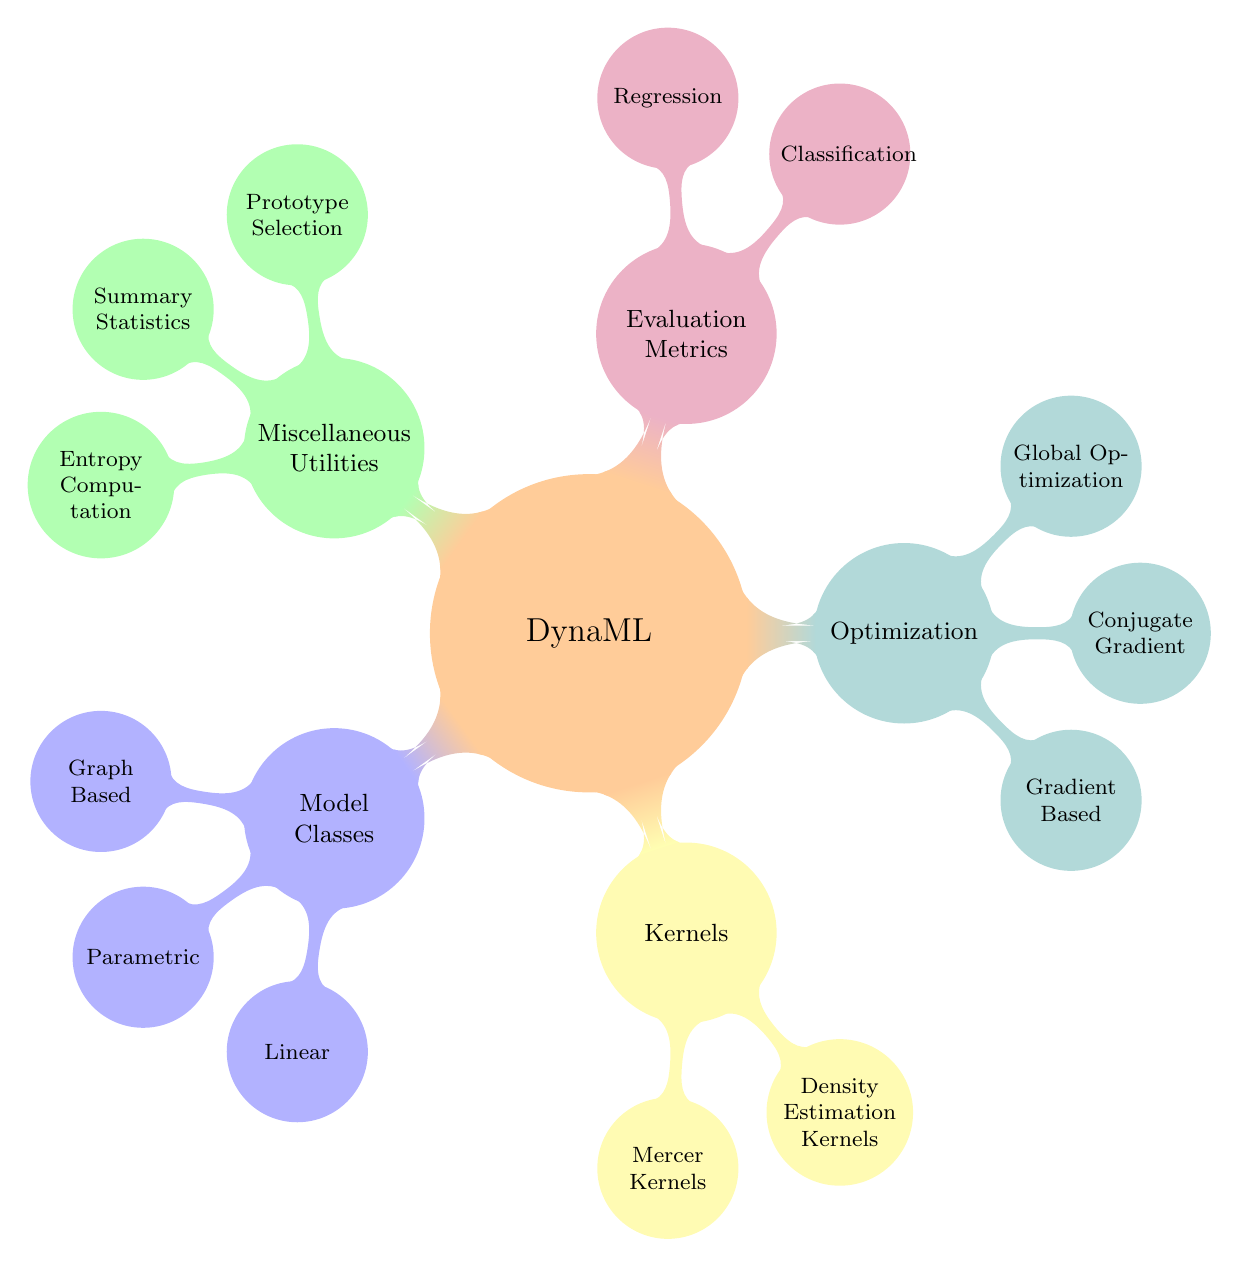
\begin{tikzpicture} [mindmap, grow cyclic, every node/.style=concept, concept color=orange!40, 
    level 1/.append style={level distance=4cm,sibling angle=72},
    level 2/.append style={level distance=3cm,sibling angle=45},]
\node{DynaML}
   child [concept color=blue!30]{ node {Model Classes}
        child { node {Graph Based}}
        child { node {Parametric}}
        child { node {Linear}}
    }
    child [concept color=yellow!30]{ node {Kernels}
        child { node {Mercer Kernels}}
        child { node {Density Estimation Kernels}}
    }
    child [concept color=teal!30]{ node {Optimization}
        child { node {Gradient Based}}
        child { node {Conjugate Gradient}}
        child { node {Global Optimization}}
    }
    child [concept color=purple!30]{ node {Evaluation Metrics}
        child { node {Classification}}
        child { node {Regression}}
    }
    child [concept color=green!30]{ node {Miscellaneous Utilities}
        child { node {Prototype Selection}}
        child { node {Summary Statistics}}
        child { node {Entropy Computation}}
    };

\end{tikzpicture}
\end{adjustbox}
\caption{Schematic structure of DynaML}
\label{fig:struct}
\end{figure}

\subsection{Class Hierarchy}

Figures \ref{fig:modelUML} and \ref{fig:modelUML1} depict the class hierarchy structures of the core and optimization modules respectively, we can discuss their role in depth.

\subsubsection*{Core Components}
The core module consists of a set of classes which all originate from a base abstraction called \textit{Model}. It also has classes \textit{ParameterizedLearner} and \textit{LinearModel} representing the core behaviors of parameter based Machine Learning models which form a large chunk of current learning techniques. By using generic typing inherent in the Scala language, one is able to separate the logic of a model from the details of the underlying data infrastructure. This is particularly relevant due to the explosion of data processing frameworks and systems like graph databases, Apache Spark, key value stores, column oriented databases, etc.

\begin{figure}[h]
\begin{adjustbox}{max width=0.5\textwidth}
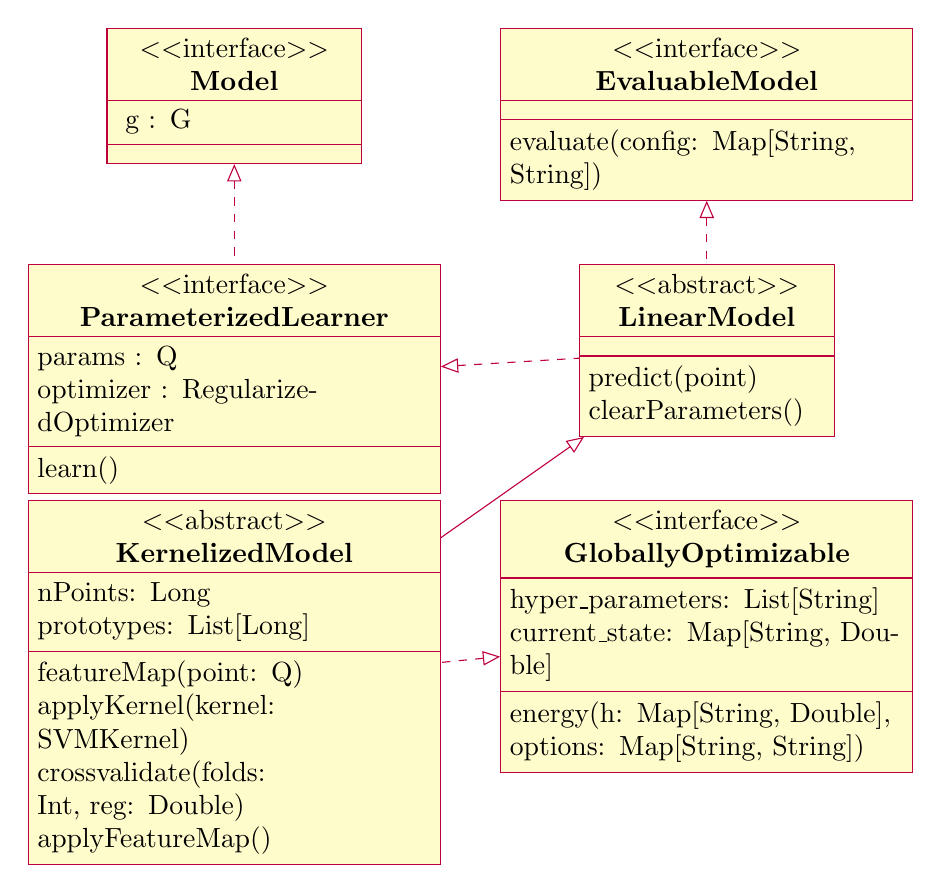
\begin{tikzpicture}
    \begin{interface}[text width =3 cm]{Model}{0 ,0}
        \attribute { g : G }
    \end{interface}
    
    \begin{interface}[]{ParameterizedLearner}{ 0 , -3}
        \implement{Model}
        \attribute{params : Q}
        \attribute{optimizer : RegularizedOptimizer}
        \operation{learn() }
    \end{interface}
    
    \begin{interface}[]{EvaluableModel}{ 6 , 0}
        \operation{evaluate(config: Map[String, String]) }
    \end{interface}
    
    \begin{abstractclass}[text width =3 cm]{LinearModel}{6 , -3}
        \implement{ParameterizedLearner}
        \implement{EvaluableModel}
        \operation{predict(point) }
        \operation{clearParameters() }
    \end{abstractclass}
    
    \begin{interface}[]{GloballyOptimizable}{ 6 , -6}
        \attribute{hyper\_parameters: List[String]}
        \attribute{current\_state: Map[String, Double]}
        \operation{energy(h: Map[String, Double], options: Map[String, String]) }
    \end{interface}
    
    \begin{abstractclass}[]{KernelizedModel}{0 , -6}
        \inherit{LinearModel}
        \implement{GloballyOptimizable}
        \attribute{nPoints: Long}
        \attribute{prototypes: List[Long]}
        \operation{featureMap(point: Q)}
        \operation{applyKernel(kernel: SVMKernel) }
        \operation{crossvalidate(folds: Int, reg: Double)}
        \operation{applyFeatureMap()}
    \end{abstractclass}
    
\end{tikzpicture}
\end{adjustbox}
\caption{Class Hierarchy of Models}
\label{fig:modelUML}
\end{figure}

\subsubsection*{Kernel Functions and Kernel Based Models}
The kernel module contains implementations of SVM kernels and AFE. The class \textit{KernelizedModel} defines kernel based linear models which use the \textit{GlobalOptimizer} class to tune values of hyper-parameters. The actual implementation of the \textit{Automatic Feature Extraction} is abstracted out in the parent classes, thereby reducing the effort of writing new SVM kernels to merely expressing their evaluation functions.

\begin{figure}[ht]
\begin{adjustbox}{max width=0.5\textwidth}
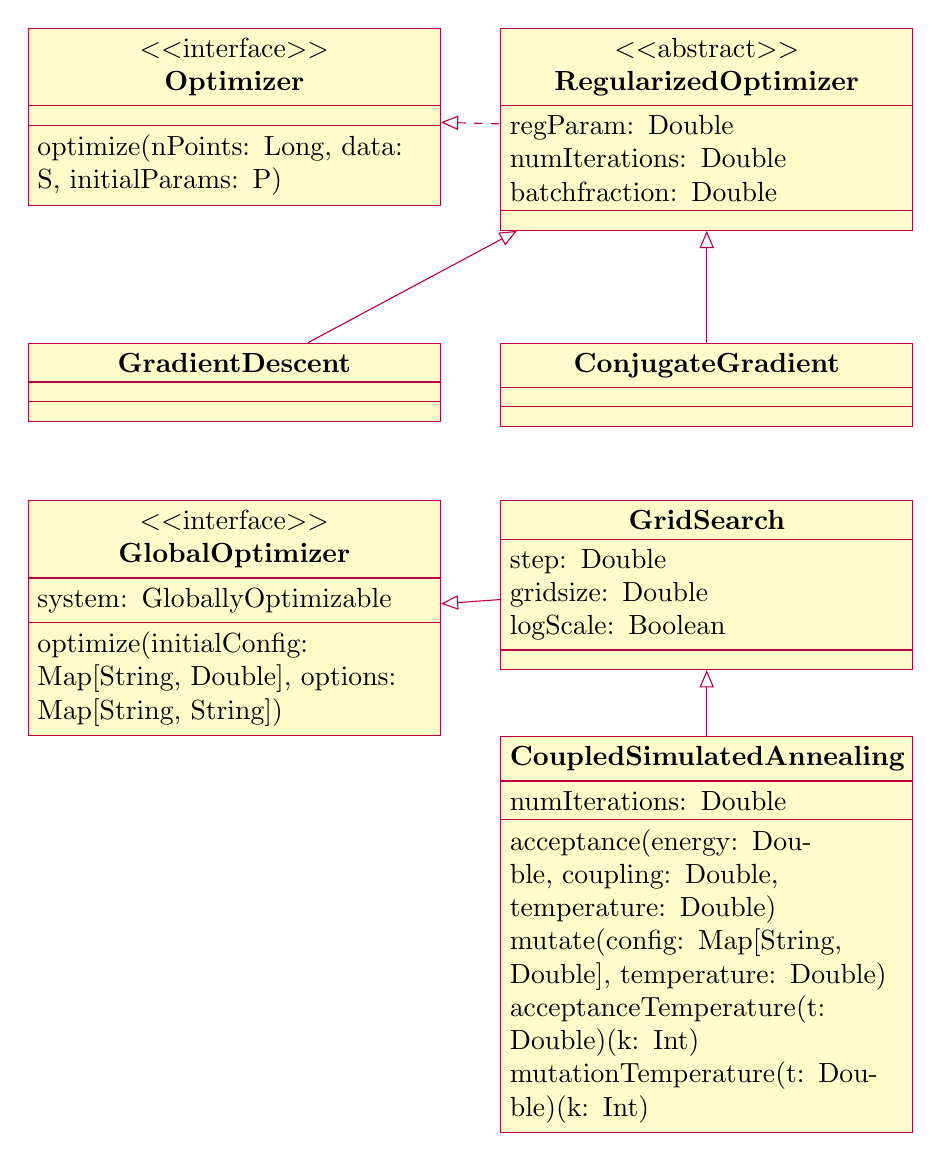
\begin{tikzpicture}
    \begin{interface}[]{Optimizer}{0 ,0}
        \operation{optimize(nPoints: Long, data: S, initialParams: P)}
    \end{interface}
    
    \begin{abstractclass}[]{RegularizedOptimizer}{6 , 0}
        \implement{Optimizer}
        \attribute{regParam: Double}
        \attribute{numIterations: Double}
        \attribute{batchfraction: Double}
    \end{abstractclass}
    
    \begin{class}[]{GradientDescent}{ 0 , -4}
        \inherit{RegularizedOptimizer}
    \end{class}
    
    \begin{class}[]{ConjugateGradient}{6 , -4}
        \inherit{RegularizedOptimizer}
    \end{class}
    
    \begin{interface}[]{GlobalOptimizer}{ 0 , -6}
        \attribute{system: GloballyOptimizable}
        \operation{optimize(initialConfig: Map[String, Double], options: Map[String, String])}
    \end{interface}
    
    \begin{class}[]{GridSearch}{6 , -6}
        \inherit{GlobalOptimizer}
        \attribute{step: Double}
        \attribute{gridsize: Double}
        \attribute{logScale: Boolean}
    \end{class}
    
    \begin{class}[]{CoupledSimulatedAnnealing}{6 , -9}
        \inherit{GridSearch}
        \attribute{numIterations: Double}
        \operation{acceptance(energy: Double, coupling: Double, temperature: Double)}
        \operation{mutate(config: Map[String, Double], temperature: Double)}
        \operation{acceptanceTemperature(t: Double)(k: Int)}
        \operation{mutationTemperature(t: Double)(k: Int)}
    \end{class}
    
    
    
\end{tikzpicture}
\end{adjustbox}
\caption{Class Hierarchy of Optimization API}
\label{fig:modelUML1}
\end{figure}

\subsubsection*{Optimization Methods}
Parametric models in DynaML have an embedded optimization object which is inherits from the \textit{Optimizer} interface. Implementations of Conjugate Gradient and Gradient Descent are provided in the optimization module. New optimization algorithms can be added by inheriting from the top level \textit{Optimizer} interface or the \textit{RegularizedOptimizer} abstract class in case one is working with parametric models which involve regularization. Another important component of the optimization module is the \textit{GlobalOptimizer} interface which acts as a skeleton for implementing gradient free global optimization algorithms.

\section{FS-LSSVM Implementation} \label{fsimpl}
The implementation of the FS-LSSVM in DynaML, outlined in algorithm \ref{lssvmalgo} is as described in the original article of Brabanter et.al \cite{DeBrabanter2010}. Kernel based models all implement the interface \textit{GloballyOptimizable} in the optimization module. Since the \textit{GlobalOptimizer} and its subclasses (i.e. \textit{GridSearch} and \textit{CoupledSimulated Annealing}) all optimize models which implement the \text{GloballyOptimizable} interface, it enables tuning of models with a variety of global optimization algorithms convenient.

\begin{algorithm} \label{lssvmalgo}
\SetAlgoLined
\KwData{Data Set, Kernel, Global Optimization routine, grid parameters}
\KwResult{Tuned FS-LSSVM model}
 Pre-process the data by mean scaling.\;
 Calculate the prototype set using iterative 
 sampling and Quadratic Renyi Entropy.\;
 Initialize a grid for the hyper-parameters\;
 \While{termination of global optimization routine}{
  Initialize the kernel using the hyper-parameters.
  Do AFE on the kernel matrix constructed from the prototypes, using the Nystrom method\;
  evaluate the cross validation score for the particular hyper-parameter values\;
 }
 \caption{Tuning FS-LSSVM}
\end{algorithm}

\section{Experiments} \label{exp}


\begin{comment}
\csvautobooktabular[tabular=|l|c|c|c|c|c|,
    table head=\hline & kernel & prototypes & globaloptimization & gridsize & gridresolution & areaunderROC\\\hline,
    late after line=\\\hline]{resultsMagicGamma.csv}{kernel=\kernel,prototypes=\prototypes,globaloptimization=\globaloptimization,gridsize=\gridsize,gridresolution=\gridresolution,areaunderROC=\areaunderROC}
{\kernel & \prototypes & \globaloptimization & \gridsize & \gridresolution & \areaunderROC}
\end{comment}

\begin{table*}[!t]
\begin{center}
\caption{Magic Gamma test results}
    \label{table1}
    \pgfplotstabletypeset[
      multicolumn names, % allows to have multicolumn names
      col sep=comma, % the seperator in our .csv file
      display columns/0/.style={
		column name=$Value 1$, % name of first column
		column type={S},string type},  % use siunitx for formatting
      display columns/1/.style={
		column name=$Value 2$,
		column type={S},string type},
	  display columns/2/.style={
		column name=$Value 2$,
		column type={S},string type},
	  display columns/3/.style={
		column name=$Value 2$,
		column type={S},string type},
	  display columns/4/.style={
		column name=$Value 2$,
		column type={S},string type},
	  display columns/4/.style={
		column name=$Value 2$,
		column type={S},string type},
      display columns/5/.style={
		column name=$Value 2$,
		column type={S},string type},
      display columns/6/.style={
		column name=$Value 2$,
		column type={S},string type},
      display columns/7/.style={
		column name=$Value 2$,
		column type={S},string type},
      every head row/.style={
		before row={\toprule}, % have a rule at top
		after row={\midrule} % rule under units
		},
		every last row/.style={after row=\bottomrule}, % rule at bottom
    ]{resultsMagicGammaProc.csv} % filename/path to file
\end{center}
\end{table*}


\section{Conclusion} \label{Conclusion}
\blindtext





% if have a single appendix:
%\appendix[Proof of the Zonklar Equations]
% or
%\appendix  % for no appendix heading
% do not use \section anymore after \appendix, only \section*
% is possibly needed

% use appendices with more than one appendix
% then use \section to start each appendix
% you must declare a \section before using any
% \subsection or using \label (\appendices by itself
% starts a section numbered zero.)
%


\appendices
% use section* for acknowledgement
\section*{Acknowledgment}



% Can use something like this to put references on a page
% by themselves when using endfloat and the captionsoff option.
\ifCLASSOPTIONcaptionsoff
  \newpage
\fi



% trigger a \newpage just before the given reference
% number - used to balance the columns on the last page
% adjust value as needed - may need to be readjusted if
% the document is modified later
%\IEEEtriggeratref{8}
% The "triggered" command can be changed if desired:
%\IEEEtriggercmd{\enlargethispage{-5in}}

% references section

% can use a bibliography generated by BibTeX as a .bbl file
% BibTeX documentation can be easily obtained at:
% http://www.ctan.org/tex-archive/biblio/bibtex/contrib/doc/
% The IEEEtran BibTeX style support page is at:
% http://www.michaelshell.org/tex/ieeetran/bibtex/
\bibliographystyle{IEEEtran}
% argument is your BibTeX string definitions and bibliography database(s)
\bibliography{sample}
%
% <OR> manually copy in the resultant .bbl file
% set second argument of \begin to the number of references
% (used to reserve space for the reference number labels box)

% You can push biographies down or up by placing
% a \vfill before or after them. The appropriate
% use of \vfill depends on what kind of text is
% on the last page and whether or not the columns
% are being equalized.

%\vfill

% Can be used to pull up biographies so that the bottom of the last one
% is flush with the other column.
%\enlargethispage{-5in}




% that's all folks
\end{document}


